\chapter{Introduction}

Asbestos is a very toxic mineral that comes in one of six types. The most common being chrysotile asbestos, which accounts for over 90\% of all the asbestos commercially used~\cite{asbestosMaacenter}. It has long, curly fibers which can be woven into materials and has many commercial applications. It is very durable, heat and chemical resistant and has strong insulating properties. These are the reasons why asbestos fibers were used in thousands of products before the toxicity became widely known. There are six main asbestos minerals that are currently regulated but there exist many more mineral forms of asbestos - mainly from the amphibole group~\cite{environmental2008framework}. The six different types are chrysotile, amosite, tremolite, crocidolite, anthophyllite and actinolite. Figure~\ref{fig:chrysotile} shows the most common form chrysotile, how it can occur in nature and how it is seen under a scanning electron microscope (SEM). \\

\begin{figure}[h]
\centering
\caption{On the left side chrysotile asbesots naturally occuring in a stone is shown~\cite{chrysoltileFullSizeImage}. On the right side two SEM images are added for comparison~\cite{mohammed2015}. The fiber like structure is very typical for chrysotile asbestos.}
\subfigure{
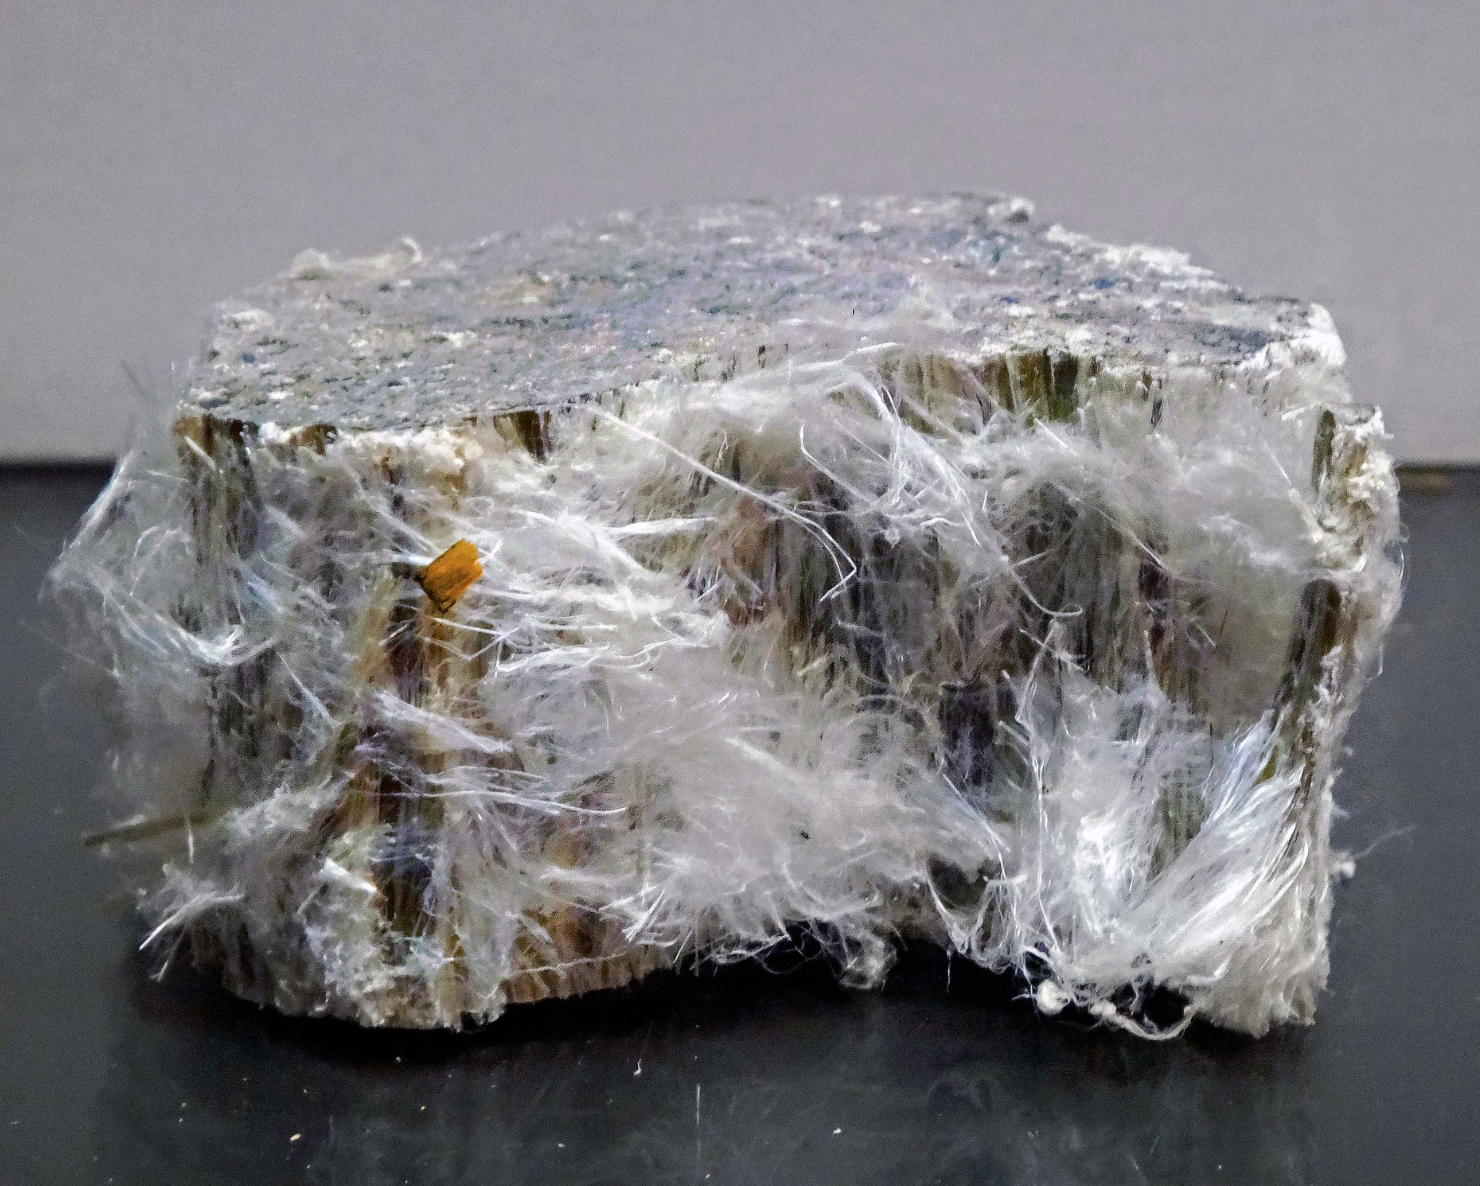
\includegraphics[width=.35\textwidth]{images/chapter1/chrysotileFullSize}
}
\subfigure{
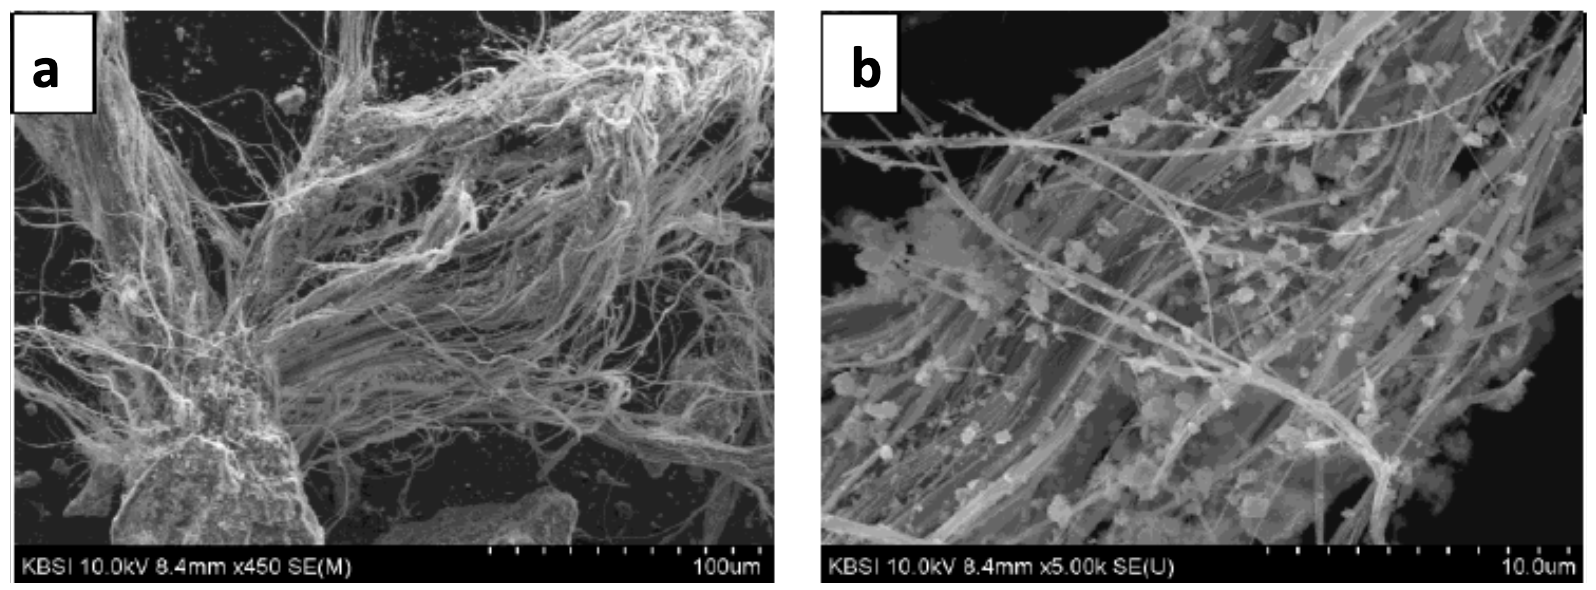
\includegraphics[width=.55\textwidth]{images/chapter1/chrysotileSEM}
}
\label{fig:chrysotile}
\end{figure}

\quad

Exposure with asbestos through inhalation or ingestion can lead to many asbestos-related diseases like mesothelioma (a type of cancer) or asbestosis (long-term inflammation and scarring of the lungs)~\cite{asbestosMaacenter, MesotheliomaWiki, asbestosisWiki}. These debilitating health effects in humans after exposure to asbestos made it very necessary to develop effective techniques and methods to detect and quantify asbestos in a variety of materials and in the environment. There is no one superior method in asbestos detection but rather a large number of different methods in preparation and analysis that need to be adapted to the specific task at hand. \\

Convolutional Neural Networks (CNNs) have become the first choice in many areas such as image recognition, classification, object detection, identifying faces and others. Although CNNs have existed already since 1988, recent progress in computational power through the immense parallelization of GPU's have made deeper and wider neural networks possible. In 2012, Alex Krizhevsky and his group won the ImageNet Large Scale Visual Recognition Challenge (ILSVRC)~\cite{krizhevsky2012imagenet, imagenet} with a CNN and since then research into this type of neural networks has increased drastically with new CNNs surpassing human-level performance in many fields. \\

A convolutional neural network is a specific type of Artifical Neural Network (ANN) which gets its name from trying to model a biological neural network. It consists of many neurons often called nodes or units that process information in a feed forward manner. A neuron receives input from other neurons (similar to brain cells that are interconnected with other brain cells) building up a huge network. This input from many different neurons is weighted and processed before forwarding the information (output) to the next neuron. A Multi Layer Perceptron (MLP) is a network consisting of fully connected layers, meaning that every neuron in one layer is connected to all the neurons in the subsequent layer. \\

For image classification, having fully connected layers of hidden units is not very useful, since no spatial information can be retrieved from the image itself. Convolutional neural networks are able to scan through the image and retrieve spatial feature maps, that find characteristic patterns throughout the image. These convolutional layers are connected to form a bigger and deeper network. These networks can be represented as directed acyclic graphs (DAGs). \\

So far, there is almost no research done on the combination of Deep Learning (DL) applied on asbestos detection from SEM images. Finding relevant publications in this field of research was very difficult at the time of writing. Although there is some work done on DL in combination with SEM images, or transfer learning applied to medical images, there is still a need to further investigate how deep learning can be used to detect asbestos fibers.\\


% It was very difficult to find publications that were relevant enough to be used for my thesis, or that came up with very original ideas to be further investigated. Although there is much research on transfer learning applied to medical images, there  is still a need to further  investigate how deep learning can be used to detect asbestos fibers.

\section{Motivation}

Asbestos detection is a very cost intensive and error prone process that needs a high degree of experience by the expert. The laboratories conducting the testing of samples need to be certified and even then, there is no guarantee that asbestos will be correctly identified. Reducing cost and error rates are important goals in order to make asbestos testing readily available, thus leading to a safer environment.\\

The motivation of this thesis is to create a model that is able to perform equally well as humans do but at a highly reduced cost; to understand how this model learns and thus increase user's trust in it; to develop strategies on how to further improve generalization and performance of the model without overfitting to the already seen data. \\

\newpage

The thesis might also inspire further research into the field of transfer learning on microscopic asbestos images and provide ideas and advice on how to achieve even better performance on this specific task.\\


\section{Study Subject}


The goal of this thesis is to study and evaluate the applicability of deep learning coupled with transfer learning to SEM images for asbestos detection. Different CNN architectures and network modifications will be investigated, transfer learning from ImageNet~\cite{imagenet} will be applied on all them and a comparison of all the different architectures with and without transfer learning will be conducted. Applying transfer learning could be challenging since the pre-trained weights are transferred from a completely different source domain. Nonetheless, it will be a central part in this thesis because only a very small dataset of asbestos images is available. Visualizations should provide important insights on what the network has learned in order to further improve on the architecture through modifications and to increase user's trust in this model. Several deep learning methods like data augmentation, cropping and dataset variations will be applied in a exploratory manner to the different architectures and their impact will be evaluated. \\

First, a good baseline needs to be established by using basic CNN architectures like AlexNet~\cite{krizhevsky2012imagenet}. The inter-rater agreement rate will additionally give a measure of how difficult it is to find mutual consensus in this task. These two metrics are the minimum requirements and further improvements will be measured against them. The current state-of-the-art architectures are all based on natural images as found in the ImageNet dataset from the ILSVRC. That raises the question if the current architectures are really optimal for the asbestos detection problem. In order to achieve good accuracies, profound understanding of the different layers of a CNN and how they interact with each other is necessary, thus providing the tools needed to perform alterations on them to increase performance while reducing complexity. Several modules in DeepDIVA~\cite{deepdiva} will need modifications and re-implementations. Transfer learning will be applied in order to start with already pre-trained weights. Fine tuning will be always performed for all layers instead of only fine-tuning the last layer.\\

The research challenge is to study the applicability of deep learning models with transfer learning from ImageNet on a very small dataset of highly specialized SEM images of asbestos.\\

\section{Microscan Service SA}

This master thesis is done in collaboration with Microscan Service SA, a certified laboratory and independent scientific center for scanning electron microscopy and microanalysis located in Lausanne, Switzerland. Microscan Service SA generously provided the dataset of SEM images of asbestos fibers used in this project. They also provided a ground truth sample of about 180 characteristic asbestos structures to learn from.

\section{Outline}

The remainder of this thesis is organized as follows. Chapter 2 explains shortly the dataset used for this task, go into related work and make an analysis of which frameworks and tools are currently used. Chapter 3 will explain CNN in detail and go through all the architectures used in this thesis and explain them. Chapter 4 will provide information on how the architectures are used and modified with the goal to increase performance at lower complexity. Several deep learning techniques are introduced and explained. Chapter 5 will evaluate transfer learning in great depth, since it is one of the main contributions of this thesis. Chapter 6 will evaluate changes to the architectures, cropping methods and dataset alterations. Chapter 7 will go into the conclusion and future work. Chapter 8 holds the Appendix with more complete visualizations and the link to the GitHub repository, where all implementation is made publicly available.\\

